\section{Overall Reflector Blocking}
\label{sec:perfect-blocking}

% Although rather extensive,
The methodology provides the basis for performing blacklist blocking
measurements at scale: a measurement technique to confidently
determine whether a reflector is blocking a particular IP address, a
viable set of reflectors that are compatible with the technique, and a
set of public security-related blacklists that provide a large set of
candidate IPs that hosts might block.  In this section, I describe my
large-scale experiment that uses this methodology for determining
which reflectors block IPs on the public blacklists, and which IPs
they block. I then present the overall results of the blocking
behavior of reflectors, and subsequent sections explore the different
behaviors in more detail.

\begin{figure}[t]
\centering
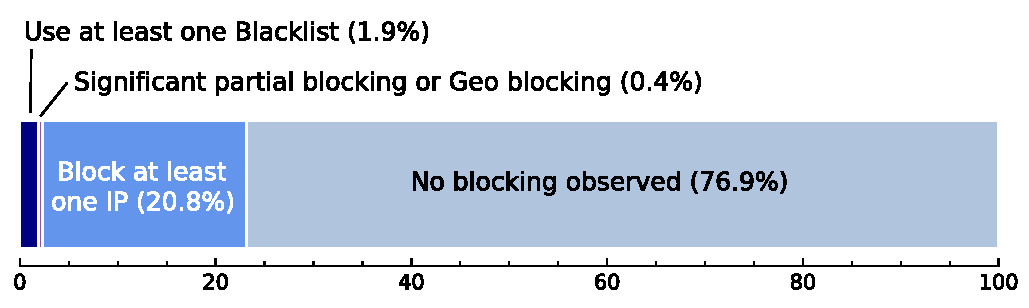
\includegraphics[width=0.95\columnwidth]{data_usage/images/reflector_breakdown_v2.pdf}
\caption{Breakdown of {\reflector} blocking based on three
  experimental runs.}
\label{fig:reflector-breakdown}
\end{figure}

For a particular experimental run, I randomly selected 25 IPs from
each blacklist that satisfies the requirements defined in
Section~\ref{sec:methodology}: exclusive, stable, routable,
geo-diversified, and AS disjoint. Then I evaluated the blocking
behavior for all {\reflroughnum} {\reflectors} against the 225
blacklist IPs sampled from all nine blacklists. To increase the chances
that these sampled IP will be stable, also to handle cases where reflectors
might update the blacklists slowly(a reflector might take a long time to
start blocking the newest IPs in a blacklist, although I discover
later that it is not the case, see Section~\ref{sec:latency-analysis}),
I ensure the sampled IPs have stayed in the blacklist for at least
2 weeks before the experiment. Since for each blacklist,
an experimental run can takes days to perform, as a post-processing step
I remove blacklist IPs from consideration that did not remain on the
blacklist for the duration of the experiment.

To increase the amount of evidence of blacklist blocking behavior, I
conducted three experimental runs, each time using a different set of 25
IPs from each blacklist. I then conclude that a {\reflector} is using a 
blacklist if only if all experiment runs show that it blocked all the 
sampled stable IPs from that blacklist.

I conducted the measurements from December 3--23rd, 2019.  During
this period, I tested 96,067,051 distinct \texttt{\small
  ({\reflector},IP)} pairs\footnote{The first two experiment I tested against
  all {\reflectors}, the last experiment I only tested against the ones that
  have shown blocking behavior in the first two tests}.
Based upon the criteria from
Section~\ref{sec:methodology}, I are able to conclusively determine
the blocking behavior (blocking or not blocking) of 98.3\% of the
tested pairs.  Among these pairs, 894,570 pairs display a
clear signal indicating ``blocking''.

Figure~\ref{fig:reflector-breakdown} presents the blocking behavior of
all 222,782 reflectors I tested partitioned into four categories:
those reflectors that I conclude use at least one of the public
blacklists (1.9\%), reflectors that block a large fraction of IPs on
at least one blacklist in every experiment(0.4\%, see more in
Section~\ref{sec:partial-blocking}), remaining reflectors that block at
least one blacklist IP (20.8\%), and reflectors that do not block any
blacklist IPs (76.9\%). (I identified 4,253 {\reflectors} that use at
  least one blacklist (Section~\ref{sec:blacklist-use}).  I also
  discovered reflectors that block a significant fraction of blacklist
  IPs, due in part to geo-blocking
  (Section~\ref{sec:partial-blocking}).  Finally, I identified a
  large number of reflectors blocking at least one IP, suggesting
  wider use of a much larger set of blacklists
  (Section~\ref{sec:large-scale}).) Note that given the requirements for hosts to
be reflectors, such as running old OS versions, it is not surprising a
large percentage shows no blocking of the blacklist IPs: they already
have attributes anti-correlated with high degrees of security hygiene.
Consequently, I want to emphasize that one should not conclude that
this percentage is representative of all hosts on the Internet.

These high-level results provide the foundation for additional
analyses and experiments, and going forward I further investigate
each of these categories of reflector blocking behavior in turn.
Section~\ref{sec:blacklist-use} explores blacklist use among the
{\reflectors}, Section~\ref{sec:partial-blocking} then examines
significant partial blocking behavior (including geo-blocking), and
Section~\ref{sec:large-scale} explores how reflectors that show any
blocking behavior can be used as evidence of much broader use of
blacklists.  As a final analysis, Section~\ref{sec:consistency}
studies the consistency of reflector blocking behavior at a coarser
granularity.

\begin{table}
\setlength{\tabcolsep}{4pt}
\centering
\caption{The number of {\reflectors} I conclude using each of the nine different
  blacklists, as well as the number of unique /24s and ASes those
  reflectors appear in.}
\begin{tabular}{l r r r}
 \toprule
 \textbf{Blacklist} (abbr.)   & \textbf{Reflectors}  & \textbf{/24s}   & \textbf{ASes}\\
 \midrule
 {\spamhausdrop} (DROP)                  & 4,142         & 1,782  & 50  \\
 {\spamhausedrop} (eDROP)                & 1,272         & 362    & 25  \\
 {\dshieldtop} (DTop)                    & 223           & 69     & 18  \\
 {\etcompromised} (ET)                   & 116           & 58     & 15  \\
 {\bdsatif} (BDS)                        & 85            & 41     & 3   \\
 {\feodo} (Feodo)                        & 64            & 26     & 16  \\
 %\textbf{\ciarmy}                              & 59            & 39 \\
 {\snortfilter} (Snort)                  & 52            & 20     & 11  \\
 {\blocklistde} (DE)                     & 36            & 18     & 8   \\
 {\ettor} (Tor)                          & 24            & 9      & 8   \\
 \midrule
 \textbf{Total Unique}                   & 4,253         & 1,827  & 77  \\
 \bottomrule
\end{tabular}

\label{tab:perfect-blocking-reflectors}
\end{table}

\section{Reflectors Using Blacklists}
\label{sec:blacklist-use}

In this section, I focus on the reflectors that use the blacklists I
study, including the relative popularity of the blacklists, patterns
in the use of multiple blacklists, and the rate at which reflectors
update.  I also use external sources of ground truth to validate my
findings.  Overall, I conclude from the results in this section that
my methodology is indeed effective at identifying blacklist use from
a remote third-party vantage point.

Recall that I use three experimental runs that test whether
reflectors block 25 randomly chosen IPs from the blacklists, and only
conclude that a reflector uses a blacklist if it blocks {\em all}
stable IPs on that blacklist across all runs.  Based on these criteria,
I identified 4,253 reflectors that use one of these public
blacklists.  Table~\ref{tab:perfect-blocking-reflectors} shows the
number of {\reflectors} using each of the nine different blacklists,
as well as the number of unique /24s and ASes those reflectors appear
in.

{\spamhausdrop} is by far the most popular blacklist in the
collection, followed by {\spamhausedrop}.  The remaining blacklists
have a comparatively small number of {\reflectors} using them.  On one
hand, since many aspects of my methodology and experiment make
conservative choices, these results should be considered a lower
bound.  On the other, one should have very high confidence in these results:
I believe these reflectors are actually on networks that block the
IPs on these blacklists.


\begin{figure}[t]
  \centering
  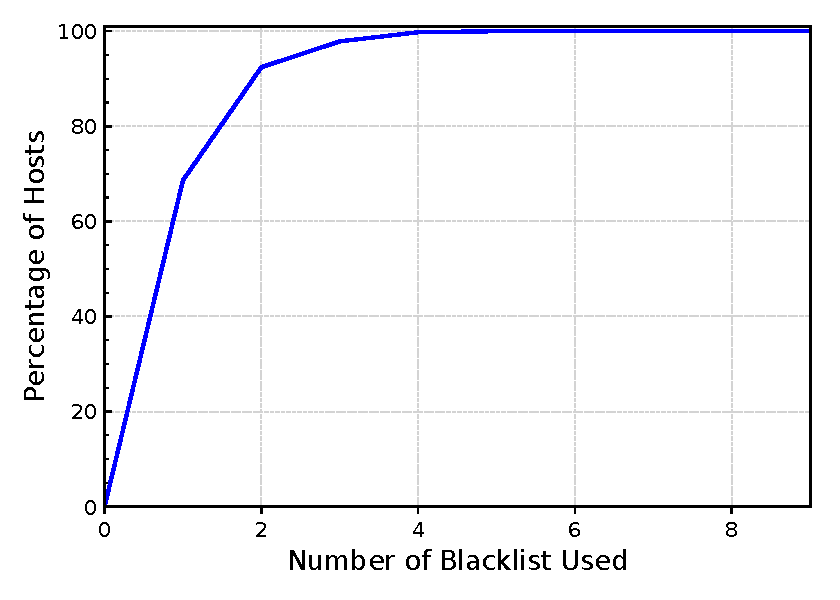
\includegraphics[width=0.8\linewidth]{data_usage/images/perfect_shared_cdf_v2.pdf}
  \caption{CDF of the number of blacklists used by {\reflectors}}
  \label{fig:perfect-shared-cdf}
\end{figure}

\subsection{Multiple Blacklist Use}

For the {\reflectors} using at least one blacklist,
Figure~\ref{fig:perfect-shared-cdf} shows the cumulative distribution
of the number of blacklists they use.  At least for the most popular
public blacklists I study, most use just one.  Over 68.6\% use just
one blacklist, 23.8\% use two or more, and only 7.6\% use three or more.
I find one {\reflector} using six of the nine blacklists -- the most
I see in my study.

For these {\reflectors}, though, there are interesting patterns to the
multiple blacklists used.  Figure~\ref{fig:perfect-heatmap} shows the
use of multiple blacklists with a heatmap.  Each cell shows the fraction of the {\reflectors} using the blacklist in the
   row $R$ that are also using the blacklist in the column $C$: $|R \cap C| / |R|$. Rows and columns
correspond to blacklists, and each cell of the heatmap shows the
fraction of the {\reflectors} using the blacklist in row $R$ that are
also using the blacklist in column $C$.  For example, the first cell
for {\etcompromised} shows that 78\% of the {\reflectors} that use ET
also use the {\spamhausdrop} blacklist.  Diagonal cells are 1.00 since
they show blacklists compared with themselves.

The first cell of the {\spamhausedrop} row indicates that all
{\reflectors} that use {\spamhausedrop} also use {\spamhausdrop}.
Since the eDROP list is an extension of the DROP list, the behavior is
strongly consistent with expectations (and, as such, is also a minor
validation of the methodology).  Moreover, the many significant values
in the first two columns show that {\reflectors} that use any of the
other blacklists very often also use {\spamhausdrop} and eDROP.  These
results underscore the popularity of {\spamhausdrop}, and indicate
that if a {\reflector} blocks traffic using blacklists, it very likely
uses {\spamhausdrop}.

\begin{figure}[t]
  \centering
  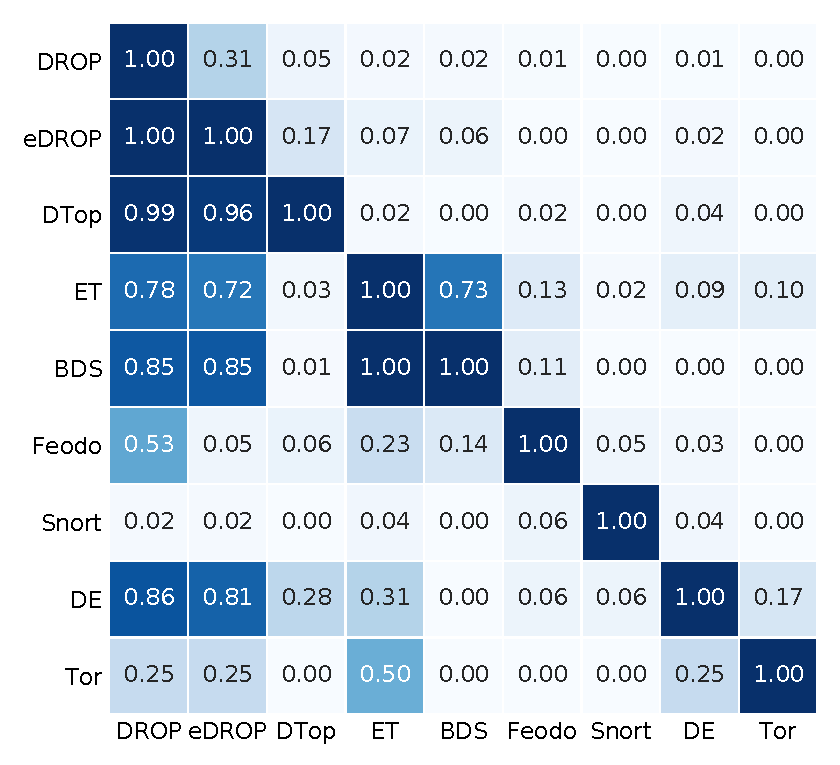
\includegraphics[width=0.85\linewidth]{data_usage/images/perfect_blocking_heatmap.pdf}
  \caption{Pair-wise overlap of {\reflectors} using the different blacklists.}
  \label{fig:perfect-heatmap}
\end{figure}
